
%associated with three attributes, i.e., workload $w$, execution rate $\sigma$, and completion time $t$.
%This makes our framework agnostic to the granularity of the resource allocation unit.
%Cores are subject to failures. We assume that core failures are independent and identically distributed (i.i.d.). We do not distinguish between soft and hard failures, assuming that soft failures are handled via software rejuvenation (i.e., rebooting \cite{466961}), while hard failures are handled by replacing the failed components with spares. We adopt the fail-stop fault model, whereby a core stops executing upon failure and failures are detected by other non-failing cores \cite{gartner_faults_1999,cristian_comm_1991}. %When a core fails, the whole execution is suspended until recovery is complete. 

%%%%%%%%%%%%%%%%%%%%%%%%%%%%%%rethinking%%%%%%%%%%%%%%%%%%%%%%
%We assume that core failures are independent and identically distributed (i.i.d.). In the real world, instead, failures are bound to be correlated. Obtaining theoretical results for non-i.i.d. failures is beyond the scope of this work. But note that one cause of correlation is the hierarchical structure of computing platforms (each rack comprises compute nodes, each compute node comprises processors, and each processor comprises cores), which leads to simultaneous failures of a group of cores. Our work applies to such failures since a group of failures can be treated as multiple individual failures that happen at the same time and their recovery can be carried out in parallel.


%We use the term core to represent the computing resource allocation unit%(e.g., a
%CPU core, a multi-core CPU, or a cluster node)
%~\cite{casanova_inria_2012}. 
%We further use $P(\sigma$, $w$, $t)$ to denote a process executing at rate $\sigma$ to complete a workload $w$ by time $t$.
The basic tenet of Lazy Shadowing is the concept of shadowing, whereby each process (\textit{main})is associated with a ``lazy" replica (\textit{shadow}) that executes at a reduced rate. 
This idea has been studied in~\cite{mills_2014_icnc} for single task and in~\cite{cui_en7085151,cui_2014_closer} for loosely-coupled MapReduce applications in the cloud environment. 
Since the target of this paper is the upcoming extreme-scale HPC systems, we introduce novel ideas that achieve efficient and scalable fault tolerance for more 
tightly coupled HPC applications (more details in Section~\ref{sec:app_model}). By carefully analyzing the characteristics of HPC applications, we devise novel ideas 
of shadow collocation and shadow leaping, and integrate them with the basic concept of shadowing, which together form a complete algorithm that we call Lazy Shadowing. 
To make it easy to follow and integrate, we first re-emphasize important details of shadowing, with minor changes of symbols.

We assume the
fail-stop failure model, where a process stops execution once a failure
occurs and failure can be detected by other
processes~\cite{gartner_faults_1999,cristian_comm_1991}.
%In order to deal with both permanent and temporary failures, the shadow process starts simultaneously with its associated main process, on a different node. Lazy Shadowing is able to tolerate any failure confined to a single node, including socket failure, CPU logical errors, bus errors, errors in the attached accelerators (e.g., GPUs), and even memory bit flips that exceed ECC's capacity. 
Under this failure model, Lazy Shadowing is able to tolerate failures in hardware, such as power supply, CPU, attached accelerators (e.g., GPU), memory bit flips that exceed ECC's capacity, and software, such as OS and runtime. 
%We only use one replica since the probability that failure occurs to both the original process and the replica is negligible~\cite{casanova_inria_2012}. %This guarantees that if one process fails, the other one can still complete the task. 
%If necessary, however, this can be easily extended to use a suit of replicas. Assuming a single failure, Lazy Shadowing can be described as follows:
The concept of Shadowing can be described as follows:
\begin{itemize}
	\item A main process, $P_m(\sigma_m$, $w$, $t_m)$, that executes at the rate of $\sigma_m$ to complete a task of size $w$ at time $t_m$.
	\item A shadow process, $P_s(<\sigma_s^b$ , $\sigma_s^a>$, $w$, $t_s)$, that initially executes at $\sigma_s^b$, and increases to $\sigma_s^a$ if its main process fails, to complete a task of size $w$ at time $t_s$.% where $\sigma_s^b$ represents the execution rate before failure, $\sigma_s^a$ the execution rate after failure, $w$ is the task size, and $t_s$ is the completion time.%, which has the same workload $w$. It starts execution simultaneously with the main process at rate $\sigma_b  \le \sigma_m$, but on a different core. Upon failure of the main process, the shadow process will be designated as the new main process, with its rate switched to $\sigma_a$ to catch up. In this case, the completion time is denoted as $t_s$. 
\end{itemize}
We only use one shadow since the probability that failures occur to both the original process and the replica is negligible~\cite{casanova_inria_2012}. 
If necessary, however, this can be easily extended to use a suit of shadows. 


%Furthermore, we adopt the
%fail-stop failure model, where a core stops execution once a failure
%occurs and failure can be detected by other
%processes~\cite{gartner_faults_1999,cristian_comm_1991}.
%In order to deal with both permanent and temporary failures, the shadow process starts simultaneously with its associated main process, on a different node. Lazy Shadowing is able to tolerate any failure confined to a single node, including socket failure, CPU logical errors, bus errors, errors in the attached accelerators (e.g., GPUs), and even memory bit flips that exceed ECC's capacity. 

Initially, the main executes at rate $\sigma_m$, while the shadow executes at $\sigma_s^b \le \sigma_m$. %To avoid simultaneous failure, they are deployed on different cores.
%with the main running at  
%a rate $\sigma_m$ and the lazy shadow at a lower rate $\sigma_s \le \sigma_m$. 
In the absence of failure, the main completes at time 
$t_m = w/\sigma_m$, which immediately triggers the termination of the
shadow. However, if at time $t_f < t_m$ the main fails, the shadow, which has completed an amount of work $w_b=\sigma_s^b * t_f$, increases its execution rate to $\sigma_s^a$ to complete the task by $t_s$. %, as depicted in Figure~\ref{fig:fail}. More specifically, the shadow completes $\sigma_s * t_f$ work by $t_f$, and finishes the remaining $(w-\sigma_s * t_f)$ work at $\sigma_a$. %The expected completion time, $T$, of the task can be easily computed by integrating $t_s(t_f) * f(t_f)$, where $f(t_f)$ is the probability of a failure occurring at time $t_f$.
The execution dynamics are depicted in Figure 1 in \cite{cui_en7085151}. %~\ref{fig:sync}.

%\begin{figure}[!t]
%	\begin{center}
%		\subfigure[Main process successful completion.]
%		{
%			\label{fig:succ}
%			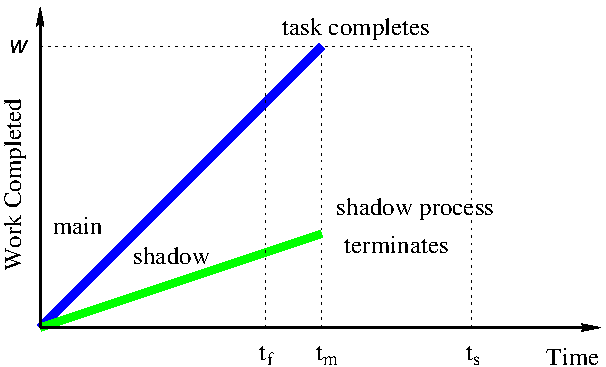
\includegraphics[width=0.7\columnwidth]{Figures/succ_new.pdf}
%		}
%		\subfigure[Main process failure.]
%		{
%			\label{fig:fail}
%			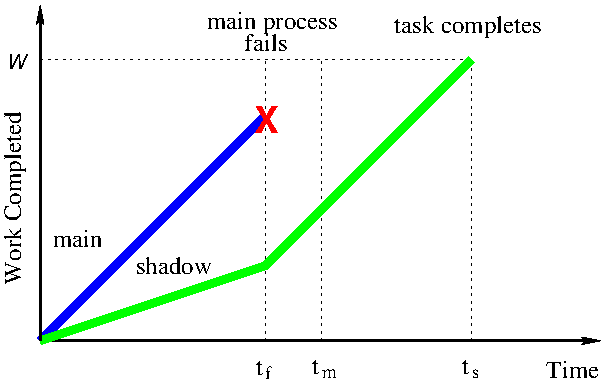
\includegraphics[width=0.7\columnwidth]{Figures/fail_new.pdf}
%		}
%	\end{center}
%	%\vskip -0.25in 
%	\caption{Lazy Shadowing execution dynamics.}
%	\label{fig:sync}
%\end{figure}

%The execution rate of the shadow before and , 

%For simplicity, we assume the maximum execution rate of a core is 1. 
In HPC, throughput consideration requires that the rate of the main, $\sigma_m$, and the rate of the shadow after failure, 
$\sigma_s^a$, be set to the maximum. 
The initial execution rate of the shadow, $\sigma_s^b$, however, can be derived by balancing the trade-offs between delay and energy.
%are determined based on the tolerance of the application to completion time.
For a delay-tolerant, energy-stringent application, $\sigma_s^b$ is set to 0, and the shadow starts executing only upon failure of the main process. %, for maximum energy saving. %, which guarantees additional energy is consumed only upon failure
For a delay-stringent, energy-tolerant application, the shadow starts executing at $\sigma_s^b=\sigma_m$ to guarantee the completion of the task at the specified time $t_m$, regardless of when the failure occurs. Therefore, Lazy Shadowing has the flexibility to converge to re-execution or process replication, if preferred. In addition,  
a broad spectrum of delay and energy tradeoffs in between can be explored either empirically or by using optimization frameworks for delay and energy tolerant applications.
%For elastic applications, the delay-energy product can be used to derive the execution rate  
%For other applications, $\sigma_s^b$ and $\sigma_s^a$ can be derived by balancing trade-offs between completion time and energy consumption
%however, may still be tuned to manage the trade-offs between completion time and energy consumption. Smaller $\sigma_b$ corresponds to lazier shadowing of the main process.

 %Figure~\ref{fig:succ} illustrates the execution scenario with no failure, while Figure~\ref{fig:fail} depicts the scenario where the main process fails.




%In terms of execution rates, this can be expressed as $\sigma_m=\sigma_a=1$ and $\sigma_s \le 1$.  




